\documentclass[a4paper,man,biblatex]{apa7}
\usepackage[american]{babel}
\usepackage{siunitx}
\usepackage[backend=biber]{biblatex}
\usepackage{float}
\usepackage{capt-of}
\usepackage[document]{ragged2e}
\setlength{\RaggedRightParindent}{0.5in}
\addbibresource{../references/references.bib}
\usepackage{graphicx}
\graphicspath{{./img/}}
\usepackage{url}
\usepackage{xpatch}
\usepackage{siunitx}
\let\paragraph\oldparagraph
\let\subparagraph\oldsubparagraph
\usepackage{titlesec, blindtext, color}

%Formatting
\titlespacing{\section}
{0pt}{-1ex}{-1ex}

\title{Streamflow Variability}
\shorttitle{}
\author{Armant Touche}
\affiliation{Portland State University}
\date{\today}

\begin{document}
%\maketitle
\noindent Name: Armant Touche\newline
\noindent Class: UNST-286D\newline
\begin{center}
    {\large Streamflow Variability}
\end{center}
\section{Introduction} 
\par  Streamflow refers to the amount of water flowing in a river at any given time in a hydrological system \autocite{streamflow_def}. The variance in streamflow differ from each region of the United States. Changes in hydrological systems, especially streamflow, in the Continental United States (CONUS) have caused some negative outcomes such as an increase in floods in some regions \autocite{rice_2016}. A regional example of a negative outcome from increased streamflow variability is the increasing number of floods in California \autocite{standford_2020}. The human "disturbance index" is measurement tool used by the United States Environmental Protection Agency (USEPA) to measure the amount of human disturbance present in watershed regions across the nation \autocite{falcone_2016}. The reason for needing the index is to use this measurement to track the past, present, and future behavior of these hydrological systems and how humans affect streamflow variation. The scale of variability is still being studied since previous methods used datasets that contained redundancies, which decreased accuracy but \textcite{falcone_2016} described the best approach to accurately classifying watershed disturbance by humans. 
\par There is a relationship between streamflow variability and both water resource availability and management \autocite{rice_2016}. For present and future studies of hydrological systems, understanding the effects of humans' activity on streamflow variability is crucial to positively manage water resources in the CONUS and elsewhere in the world.\\
\section{Data Analysis}  
\par First, some regional examples in the CONUS of streamflow variability effects. To better understand the negative outcomes from increased streamflow variability and increasingly changing climate, the \textcite{mallakpour_2018} study reported streamflow minimum and maximum annual streamflows mean (\si{\cubic\meter\per\second}) trends in various watersheds in Northern California.\\ 
\par In \textit{Figure 1}, notice the minimum streamflow values (red-down arrows) in panels (D-F). In D-panel, there are more reports on negative trends occurring in streamflow values from 1950-2005 which means that inland streams are displaying a decreasing mean during the dry seasons and in G-panel, during the wet season, there is an increase in the mean streamflow value. The increase in streamflow mean during the wet-season promotes more floods and a decrease in mean during dry-season promotes more droughts \autocite{mallakpour_2018}. Although the trends are minor from 1950-2005, the cumulative distribution for future trends highlight a negative trend. Cumulative distribution is likelihood or probability for a non-discrete value to occur at any given point ranging from one to zero, usually referred to as a random variable. In the current context, the random variable is streamflow discharge (\si{\cubic\meter\per\second}) \autocite{cdf_def}.\\
%Fig. 1
 \begin{minipage}{0.5\linewidth}   
     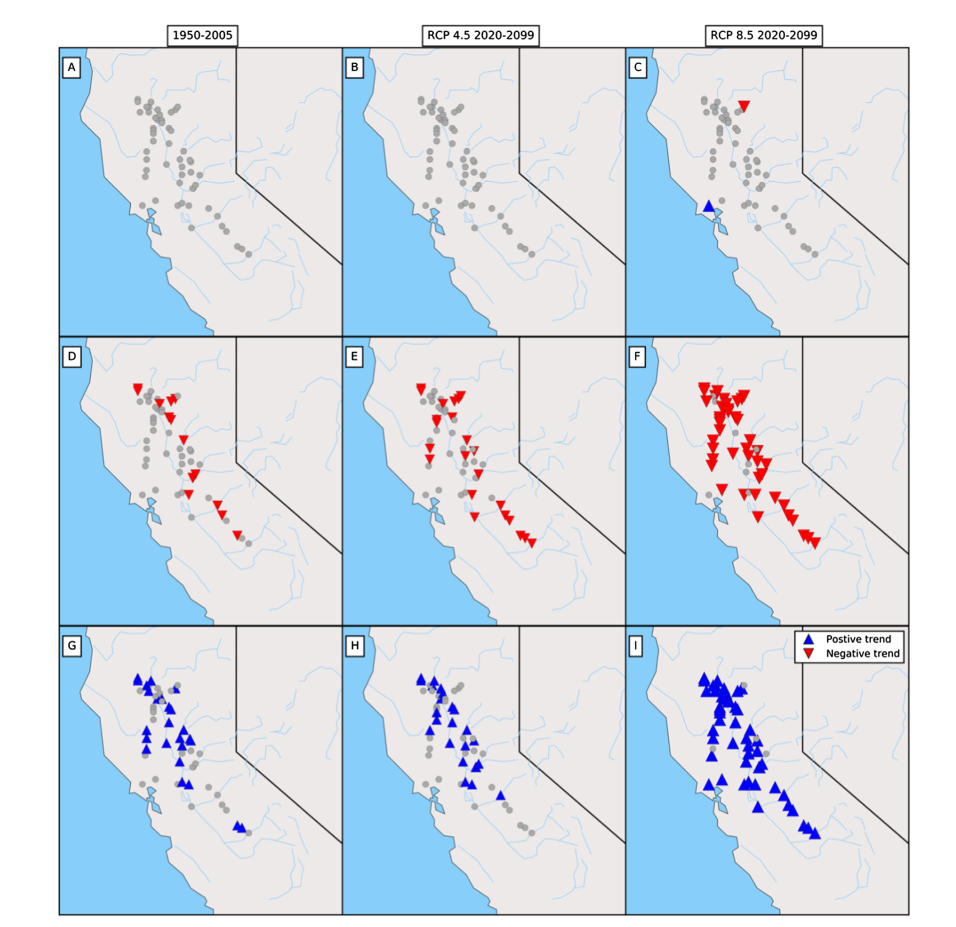
\includegraphics[scale=0.4]{stream_flow_cali.png}
     \captionof{figure}{\autocite{mallakpour_2018}}
     \label{fig:streamflow_trend}
\end{minipage}
\vspace{1ex}
\par \textit{Figure 2} highlights cumulative trend which displays the cumulative distribution of three datasets -- (1) 1950-2005 (2) Representative Concentration Pathway (RCP) 4.5 2020-2099 (3) RCP 8.5 2020-2099. The left panel is Oroville Lake in California and the right panel is Shasta Lake. Notice the blue line's distribution is greater than the two project trends from RCP 4.5 and RCP 8.5. RCP 4.5 is a model of future streamflow trends which uses a bias-corrected projection on data derived from global climate model (GCM) and RCP 8.5 also uses data derived from GCM to simulate future streamflows trends. GCM data is known to have systematic error (biases) due to limited GIS spatial resolution which is why one (RCP 4.5) of the two future projections uses a bias correction projection to account for theses errors (biases).\\
%Fig. 2
\begin{minipage}{0.5\linewidth}   
    \centering
    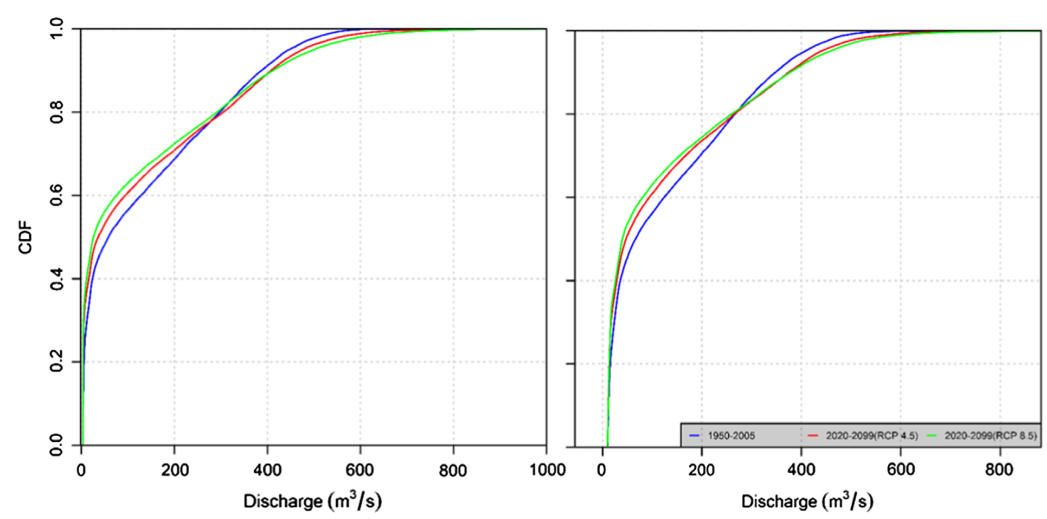
\includegraphics[scale=0.40]{cdf_streamflow.png}
    \captionof{figure}{Empirical Cumulative Distribution Functions (ECDFs) \autocite{mallakpour_2018}}
\end{minipage}
\par But how does climate change affect streamflow variability? From \textcite{rice_2016} study, atmospheric variables may be potential drivers in streamflow variability. \textcite{rice_2016} results suggest that human activities may magnify or amplify the expression of changes. $P_\textit{mean}$ (mm) and $DI_\textit{mean}$ (Soil Dryness index) which were the important atmospheric variables that acted as drivers. There were more variables being used by United State Geological Survey (USGS) but watershed climatology, for instance was too varied amongst CONUS watersheds. \textit{Figure 3} models streamflow trends across the CONUS \autocite{rice_2016}. The red markers depict a decreasing trend in streamflow mean values and blue depicts an increase in streamflow mean values. Again, drawing our notice to the Southwest region, the increased number cases of floods in California highlights the relationship with the blue markers which model increased streamflow variability. \\
%Fig. 3
 \begin{minipage}{0.5\linewidth}   
     \centering
    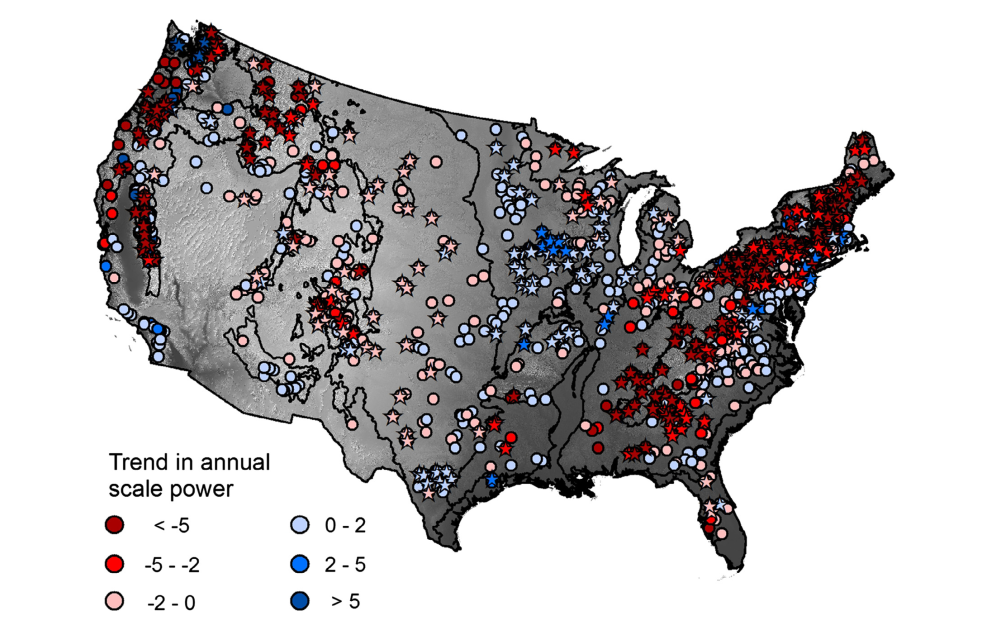
\includegraphics[scale=.4]{conus_trend}
    \captionof{figure}{\protect\autocite{mallakpour_2018}}
\end{minipage}
\section{Results}
\par To understand how human activity contributes to streamflow variability within streams, let's discuss the human "disturbance index" mentioned in \textcite{falcone_2016} study. Building roads, damming streams, and inputs from agricultural sources and urban sources serve as contributors to changes in stream ecosystems. \textcite{falcone_2016} was not the only study to try to measure human activity. In \textcite{stein_2002}, they mentioned that previous studies used biological markers as a way of measuring human activity (i.e. soil sampling and other biological harvesting methods) which can be time consuming and are site-specific. The sample from one site does not necessarily mean that it represent the whole. Still, the duty of monitoring human effects of environment should be a priority when it comes to urban and landscape planning \autocite{stein_2002}. With the advent of the Geographic Information System (GIS), better data can be derived which uses multiple variables versus the single variable approach described in \textcite{stein_2002} and other studies \autocite{falcone_2016}. The biggest take away from \textcite{falcone_2016} is that a reduced variable set can reproduce inferences from different watershed sites and the main six variables that should be used to measure human's impact on streams are: (1) housing-unit density (housing unit \si{\per\square\kilo\meter}), (2) Road density in watershed (\si{\kilo\meter\per\square\kilo\meter}), (3) Sum of 43 major pesticide compounds (\si{\kilo\gram\per\square\kilo\meter}), (4) Urban-crops-pasture land cover in a 600 m mainstem buffer, (\%), (5) Average linear distance of sampling site to all canals/ditches (m), (6) Dam storage in basin (liters $\times$ 1000 \si{\square\kilo\meter}). 
\par Although the focus can be centered around these variables, there is still an issue with deriving GIS data on small-to-medium sized watersheds. The reason for difficultly is that the resolution is sometimes too low for accurate spatial analysis hence why the variables are not to reliant on variables involving spatial quantities. Examples of spatial quantities are most of the variables from the National Land Cover Data-set \autocite{falcone_2016}. Even with resolution errors, the results from this study suggest that "disturbance index" is an objective, deductionist approach to measuring humans activities' effect on streamflow. The data analysis conducted by \textcite{mallakpour_2018} suggests that anthropogenic effects are affecting streamflow  and will continue effecting hydrologically systems like the watersheds in Northern California.\\
\section{Discussion} Water and climate change are quickly becoming global and political issues and many of these issues relate with national security and human health. Before the 70's, obtaining topological images without the aide of computers was a chore that many scientists did not like to do. Even after receiving images or maps, the accuracy may not or may have been the best because of the decentralized nature of information and standards back then. With better systems for acquiring maps, like the Internet, has boosted research interests into hydrological systems in order to understand water and climate change issues \autocite{bras_1999}. In \textcite{bras_1999} article, he believes the studies of groundwater hydrology increased scientists' interest into studying the impact of certain variables that affect certain properties with hydrology, particularly flow and transport.\\
\section{Conclusion} The results from \textcite{rice_2016} conclude that climate change does and has affected streamflow in CONUS which serve as sources for freshwater. Using indexes like the "disturbance index" mentioned in \textcite{falcone_2016} can objectively quantify the impact from human activity like urban developing and water flow controls. It's no wonder that the CONUS is experiencing more droughts in some areas like the Pacific Northwest and more floods in areas like Southern California. The usage of GIS-derived data can be prone to errors like low pixel resolution on small-to-medium watersheds but still, the "disturbance index" is a useful \textit{a priori} method for measuring anthropogenic effects on streamflow. 
\par Future streamflow models predict increasing variability in streamflow. Increased variability will further complicate  water resource management in the CONUS and elsewhere in the world. Not only complicate water management but will also cause more floods and droughts as mentioned the data analysis performed by \textcite{mallakpour_2018}. In order to combat this difficult task, studies need to standardize what activites affect hydrological systems which are mainly the six variables mentioned in \textcite{rice_2016}. The variables that deserve to be highlighted are: (1) housing-unit density (housing unit \si{\per\square\kilo\meter}), (2) Road density in watershed (\si{\kilo\meter\per\square\kilo\meter}), (3) Sum of 43 major pesticide compounds (\si{\kilo\gram\per\square\kilo\meter}), (4) Urban-crops-pasture land cover in a 600 m mainstem buffer, (\%), (5) Average linear distance of sampling site to all canals/ditches (m), (6) Dam storage in basin (liters $\times$ 1000 \si{\square\kilo\meter}). I feel confident that more studies are being had based on information stated in the data on sources section part of the appendix. The data from research on the sources suggests that there are more studies that are newer than 2017 taking place versus studies before 2017.

\printbibliography

%Appendix 
\appendix
\section{Data On Sources}
\label{appendix:data_on_source}

\begin{enumerate}

    %1
    \item \textcite{rice_2016} - \textit{Influence of watershed}...
        \begin{enumerate}
            \item Search engine used: \url{https://search.library.pdx.edu/primo-explore/}
            \item Keywords: "streamflow variability"AND"human activity"
            \item How many results: 8 
            \item How many were peer-reviewed: 8
            \item How many are from 2017 or newer: 5
            \item Calculate \% new peer-reviewed $62.50$  \%
            \item Link: \url{https://www-sciencedirect-com.proxy.lib.pdx.edu/science/article/pii/S002216941630436X}
            \item Type: Peer-reviewed article
        \end{enumerate}

    %2
    \item National Institute of Standards and Technology (NIST) - \textit{Related Distribution}
        \begin{enumerate}
            \item Search engine used: Google
            \item Keywords: Cumulative Distribution website:gov
            \item How many results: $3.25\times 10^8$
            \item How many were peer-reviewed:  N\textbackslash A
            \item How many are from 2017 or newer: N\textbackslash A
            \item Calculate \% new peer-reviewed: N\textbackslash A 
            \item Link: \url{https://www.itl.nist.gov/div898/handbook/eda/section3/eda362.htm}
            \item Type: Reference 
        \end{enumerate}

        
    %3
    \item \textcite{stein_2002} - \textit{Spatial analysis of anthropogenic}...
        \begin{enumerate}
            \item Search engine used: Discovered source within \textcite{falcone_2016}
            \item Keywords: N\textbackslash A 
            \item How many results: N\textbackslash A
            \item How many were peer-reviewed: N\textbackslash A
            \item How many are from 2017 or newer: N\textbackslash A
            \item Calculate \% new peer-reviewed: N\textbackslash A
            \item Link: \url{https://www-sciencedirect-com.proxy.lib.pdx.edu/science/article/pii/S0169204602000488}
            \item Type: article 
        \end{enumerate}


    %4
    \item United States Geological Survey (USGS) - \textit{Streamflow and Water Cycle}
        \begin{enumerate}
            \item Search engine used: Google
            \item Keywords: streamflow overview website:gov 
            \item How many results: $5.6\times 10^5$
            \item How many were peer-reviewed: N\textbackslash A
            \item How many are from 2017 or newer: N\textbackslash A
            \item Calculate \% new peer-reviewed: N\textbackslash A 
            \item Link: \url{https://www.usgs.gov/special-topic/water-science-school/science/streamflow-and-water-cycle?qt-science_center_objects=0#qt-science_center_objects}
            \item Type: reference 
        \end{enumerate}


    %5
    \item \textcite{mallakpour_2018} - \textit{A new normal for} ... 
        \begin{enumerate}
            \item Search Engine used: PSU library search engine
            \item Keywords: southern california stream variability
            \item How many results: 59,973 
            \item How many were peer-reviewed: 16,308
            \item How many are from 2017 or newer: 8,038
            \item Calculate \% new peer-reviewed 49.29\%
            \item Link: \url{https://www-sciencedirect-com.proxy.lib.pdx.edu/science/article/pii/S0022169418307844}
            \item Type: article 
        \end{enumerate}

    % 6
    \item \textcite{falcone_2016} - \textit{Quantifying Human disturbance}
        \begin{enumerate}
            \item Search Engine used: PSU library search engine
            \item Keywords: Discovered source within \textcite{rice_2016} article
            \item How many results: N\textbackslash A 
            \item How many were peer-reviewed: N\textbackslash A
            \item How many are from 2017 or newer:  N\textbackslash A
            \item Calculate \% new peer-reviewed: N\textbackslash A
            \item Link: \url{https://www-sciencedirect-com.proxy.lib.pdx.edu/science/article/pii/S1470160X09000983}
            \item Type: article 
        \end{enumerate}

    %7
    \item \textcite{bras_1999} - \textit{A  Brief  History  of  Hydrology}
        \begin{enumerate}
            \item Search engine used: Google
            \item Keywords: history of hydrology 
            \item How many results: $1.83\times 10^8$ 
            \item How many were peer-reviewed: N\textbackslash A
            \item How many are from 2017 or newer:  N\textbackslash A
            \item Calculate \% new peer-reviewed: N\textbackslash A
            \item Link: \url{https://journals.ametsoc.org/doi/pdf/10.1175/1520-0477-80.6.1151}
            \item Type: article 
        \end{enumerate}

    %8
    \item \textcite{standford_2020} - \textit{More rain and less snow}...
        \begin{enumerate}
            \item Search engine used: Google
            \item Keywords: Southern California flooding 
            \item How many results: $2.69\times 10^8$ 
            \item How many were peer-reviewed: N\textbackslash A
            \item How many are from 2017 or newer:  N\textbackslash A
            \item Calculate \% new peer-reviewed: N\textbackslash A
            \item Link: \url{https://news.stanford.edu/2020/01/27/rain-less-snow-increases-flooding/}
            \item Type: news article 
        \end{enumerate}
    
    

\end{enumerate}

\end{document}
